\documentclass[a4,landscape]{article}
\usepackage{tikz}

\begin {document}

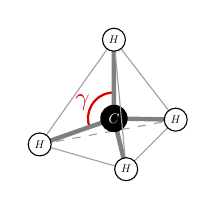
\begin{tikzpicture}

%Metaani

%Tetraedri
\draw[gray!75, dashed] (-0.943,-0.33,0) coordinate (b) -- (0.47,-0.33,-0.817) coordinate (d);
\draw[gray!75] (0,1,0) coordinate (a)  -- (b) -- (0.47,-0.33,0.817) coordinate (c)  -- (d) -- cycle;

%Sidoskulma
\draw[thick, red!85!black] (0,.33,0) arc (90:199.5:.33);
\node[scale=.9] at (-.4,.2,0) {$\textcolor{red!90!black}\gamma$};


%Atomit ja sidokset
\draw[ultra thick, gray] (a) -- (0,0,0) coordinate (O) -- (b);
\draw[ultra thick, gray](c) -- (O) -- (d);
\node[circle, fill=black, scale = 0.5] at (O) {$\textcolor{white}C$};
\draw [gray!75] (a) -- (c);
\foreach \v in {a, b, c, d}
	\node[circle, draw=black, fill=white, scale = 0.4] at (\v) {$H$};


\end{tikzpicture}

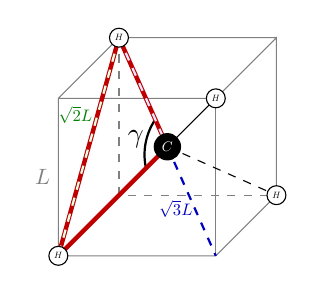
\begin{tikzpicture}

%Kuutio
\draw[gray] (-1,1,1) coordinate (A) -- (1,1,1) coordinate (B) -- (1,1,-1) coordinate (D) -- (1,-1,-1) coordinate (H) -- (1,-1,1) coordinate (F) -- (-1,-1,1) coordinate (E) -- (A)  -- (-1,1,-1) coordinate (C) -- (1,1,-1) coordinate (D);
\draw[gray]  (B) -- (F);
\draw[gray, dashed] (C) -- (-1,-1,-1) coordinate (G) -- (H);
\draw[gray, dashed] (E) -- (G);

% Sidoskulma
\draw[thick] (-.25,.25,-.25) arc (146:194:.8);
\node at (-.4,.1,0) {$\gamma$};

% Tarkasteltava kolmio
\draw[ultra thick,red!75!black] (C) -- (0,0,0) coordinate (O) -- (E) -- cycle;

% Sivun pituus
\node[scale=0.8] at (-1.2,0,1) {$\textcolor{gray}L$};

% Tahkon lävistäjä
\draw[thick, dashed, green!10] (C) -- (E);
\node[scale = 0.6] at (-.975,.6,.5){$\textcolor{green!50!black}{\sqrt 2 L}$};

% Kuution lävistäjä
\draw[thick, dashed, blue!10] (C) -- (O);
\draw[thick, dashed, blue!75!black] (O) -- (F);
\node[scale = 0.6] at (0.3,-.6,.5){$\textcolor{blue!75!black}{\sqrt 3 L}$};

%Metaani
\draw[dashed](0,0,0) coordinate (O) -- (H);
\draw (O) -- (B);
\node[circle, fill=black, scale = 0.5] at (O) {$\textcolor{white}C$};
\foreach \v in {C, B, E, H}
	\node[circle, draw=black, fill=white, scale = 0.33] at (\v) {$H$};

\end{tikzpicture}

\end{document}